\documentclass[conference]{IEEEtran}
\IEEEoverridecommandlockouts
% The preceding line is only needed to identify funding in the first footnote. If that is unneeded, please comment it out.
\usepackage{ctex}
\usepackage{cite}
\usepackage{amsmath,amssymb,amsfonts}
\usepackage{algorithmic}
\usepackage{graphicx}
\usepackage{textcomp}
\usepackage{xcolor}
\usepackage{listings}
\usepackage{float}

\lstset{basicstyle=\small\fontencoding{T1}\ttfamily,breaklines=true}
\lstset{frame=shadowbox,tabsize=4}

\def\BibTeX{{\rm B\kern-.05em{\sc i\kern-.025em b}\kern-.08em
    T\kern-.1667em\lower.7ex\hbox{E}\kern-.125emX}}
\begin{document}

\title{
	基于 CycleGAN 的风格迁移的设计与实现
}

\author{
\IEEEauthorblockN{王凯祺 \ 16337233}
\and
\IEEEauthorblockN{李洋 \ 16337124}
\and
\IEEEauthorblockN{李伟基 \ 16337122}
}

%\author{\IEEEauthorblockN{1\textsuperscript{st} Chongxuan Li}
%\IEEEauthorblockA{\textit{Dept. of Comp. Sci \& Tech.} \\
%Tsinghua University, Beijing, 100084, China \\
%licx14@mails.tsinghua.edu.cn}
%\and
%\IEEEauthorblockN{2\textsuperscript{nd} Kun Xu}
%\IEEEauthorblockA{\textit{TNList Lab} \\
%Tsinghua University, Beijing, 100084, China \\
%xu-k16@mails.tsinghua.edu.cn}
%\and
%\IEEEauthorblockN{3\textsuperscript{rd} Jun Zhu}
%\IEEEauthorblockA{\textit{State Key Lab of Intell. Tech. \& Sys.} \\
%Tsinghua University, Beijing, 100084, China \\
%dcszj@mail.tsinghua.edu.cn}
%\and
%\IEEEauthorblockN{4\textsuperscript{th} Bo Zhang}
%\IEEEauthorblockA{\textit{Center for Bio-Inspired Computing Research} \\
%Tsinghua University, Beijing, 100084, China \\
%dcszb@mail.tsinghua.edu.cn}
%}

\maketitle

\begin{abstract}
风格迁移是一类视觉与图形的问题。它的工作原理是用成对的图像作为训练集,学习输入图像到输出图像之间的映射。然而,对于很多任务来说,我们很难准备成对的图像作为训练集。因此我们提供一种方法,使得能在没有成对图像训练集的情况下,仍能从一张在源集合 $X$ 中的图片转化为目标集合 $Y$ 中的图片。我们的目标是学习一种映射 $G: X \rightarrow Y$ ,使得用对抗性损失函数无法区分 $G(X)$ 的分布与 $Y$ 的分布。单纯考虑单一的映射 $G$ 会使问题难以解决,我们将映射 $G$ 和它的逆映射 $F: Y \rightarrow X$ 结合起来,并引入循环一致性损失函数来保证 $F(G(X)) \approx X$ 且 $G(F(X)) \approx X$。用这样的方法结合生成对抗网络,即可完成风格迁移的任务。
\end{abstract}


\section{前言}

生成对抗网络在图像生成、图像处理中扮演着关键的角色,而风格迁移又是当前比较热门的话题。那是否存在一种方法,把生成对抗网络与风格迁移结合起来,即用生成对抗网络来解决风格迁移问题。在本文中,我们将展示一种风格迁移的方法:从一个图像集合中提取一些特征(风格),然后指出如何从这些特征翻译成另一个图像集合中的特征。

风格迁移问题在广义上可以被表示为图像到图像的翻译问题,即给定一个图像在特定场景(记为 $x$ )下的表示,我们需要将它转化为另一个场景 $y$ 下的表示,例如从相机拍的图像转化成彩铅图像。采用计算机视觉、图像处理技术,我们可以在有监督学习的条件下用成对的图像 $\{x_i, y_i\}_{i=1}^{N}$ (如图 \ref{l1} ) 建立起一套强大的图像翻译系统。但是,获取成对的训练数据是非常困难的,也非常昂贵。例如,像语义分割等任务,只存在几个数据集,它们相对较小。要获得艺术风格化类图形任务的输入输出对可能更加困难,因为期望输出更加困难,因为期望输出非常复杂,通常需要艺术创作。

\begin{figure}
\centering
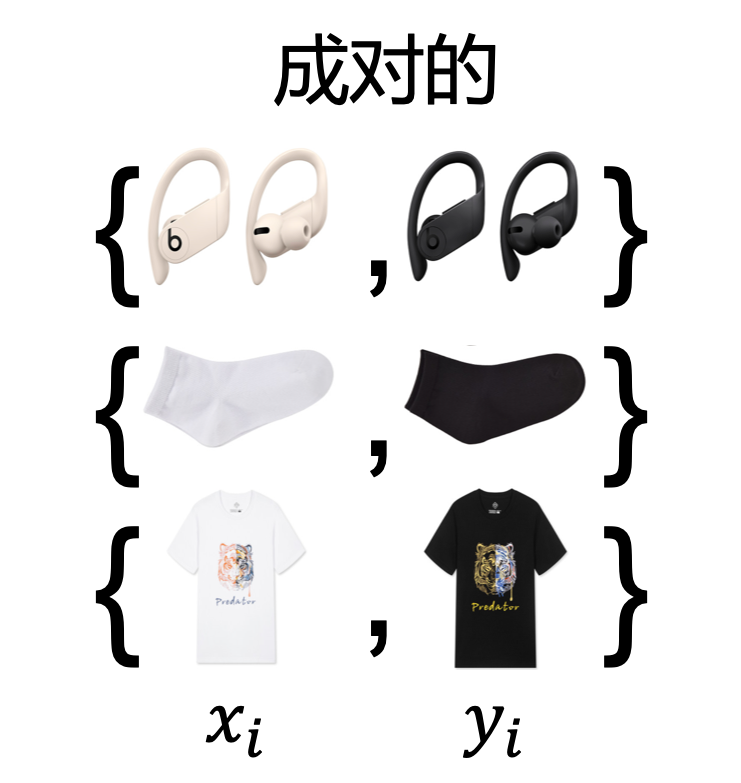
\includegraphics[scale=0.5]{img/1.png}
\caption{成对的训练数据包含 $N$ 个样本 $\{x_i, y_i\}$ ,其中 $x_i$ 和 $y_i$ 是成对的。}
\label{l1}
\end{figure}

因此,我们需要设计一种算法,可以在没有输入输出对的情况下在图像域之间进行转换(如图 \ref{l2} 右侧)。我们假设域之间存在一些潜在的关系(如两张图片是同一个场景的不同渲染结果),并且我们希望学习这种关系。虽然我们缺乏在配对层面上的监督,但我们可以在集合层面进行监督:在域 $X$ 中给定一组图像,在域 $Y$ 中给定另一组图像。我们可以训练一个映射 $G: X \rightarrow Y$ 使得输出 $\hat{y} = G(x), x \in X$ 和 $Y$ 集合中的图像 $y$ 无法被判别器(用于区分 $\hat{y}$ 与 $y$ 的模型)区分。理论上,映射 $G$ 可以在 $\hat{y}$ 上产生与经验分布相匹配的输出分布 $p_{data}(y)$ 。最终,最优的映射 $G$ 将域 $X$ 转换成与 $Y$ 相同分布的域 $\hat{Y}$ 。但是,由于有无数的映射 $G$ 会在 $\hat{y}$ 上产生相同的分布,这种转换并不能保证单个输入 $x$ 和输出 $y$ 是成对的。此外,在实践中,我们发现很难单独优化对抗性目标:标准的训练过程会导致模型崩溃,模型直接将输入图像映射到相同的输出图像。

\begin{figure}
\centering

\includegraphics[scale=0.5]{img/2.png}
\caption{不成对的训练数据包含一个源集合 $\{x_i\}_{i=1}^{N}(x_i \in X)$ 和一个目标集合 $\{y_i\}_{j=1}^{M}(y_i \in Y)$ ,并且不提供额外的信息如哪个 $x_i$ 与哪个 $y_j$ 成对。}
\label{l2}
\end{figure}

这些问题需要我们在目标上添加更多结构。我们应该利用翻译的循环一致性,比如说,一个句子从中文翻译成英文,再从英文翻译成中文,我们应该得到与原来一样的句子。在数学上说,如果我们有一个翻译器 $G: X \rightarrow Y$ 和另一个翻译器 $F: Y \rightarrow X$ ,那么 $G$ 和 $F$ 必须互为对方的逆,并且两个映射都应该是双映射。为了满足这个假设,我们可以同时训练这两个映射 $G$ 和 $F$ ,并用“循环一致性损失函数”来保证 $F(G(x)) \approx x$ ,且 $G(F(y)) \approx y$ 。把这个损失与在域 $X$ 和 $Y$ 上的对抗性损失结合起来,我们就可以实现在没有成对图像的训练集中,进行图像到图像的翻译。

我们把这种方法应用到风格迁移,并与前人的实验作比较。我们的方法比前人的方法无论是在速度上还是质量上都有优势。

\section{相关工作}

\paragraph{生成对抗网络(GAN)\cite{b16}}
生成对抗网络在图像生成 \cite{b6}、图像编辑 \cite{b66} 等领域取得极好的效果。生成对抗网络成功的关键在于对抗性损失的想法,这种对抗性损失使得在理论上,生成的图像与真实的照片无法区分。这种损失对于图像生成任务非常有用,也因此成为计算机图形学中优化的目标。我们采用对抗性损失来学习映射函数,让翻译的图像无法与目标域中的图像区分。

\paragraph{循环一致性}
很久以前,就已经有人使用传递性作为规范结构化数据的方法。 在视觉跟踪领域,保证简单的前后一致性已成为数十年的标准技巧 \cite{b24} \cite{b48} 。在我们的实验中,我们引入了循环一致性损失函数,来保证映射 $G$ 和 $F$ 相互一致。

\paragraph{神经网络风格迁移 \cite{b13} \cite{b23}}
前人用深度神经网络构建了一套人工系统,用于创建高感知质量的艺术图像。该系统使用神经表示来分离和重新组合任意图像的内容和风格,为艺术图像提供神经网络算法。它对风格迁移问题的求解思路跟我们使用生成对抗网络的求解思路完全不同。我们将它的算法与我们的算法进行对比。



\section{研究问题的定义}

我们的目标是给定训练样本 $\{x_i\}_{i=1}^{N}$ 和 $\{y_i\}_{j=1}^{M}$ ,其中 $x_i \in X, y_j \in Y$ ,然后学习 $X$ 到 $Y$ 的映射。我们将数据分布表示为 $x \sim p_{data}(x)$ 和 $y \sim p_{data}(y)$  。在图?中可以看到,我们的模型包含两个映射 $G: X \rightarrow Y$ 和 $F: Y \rightarrow X$ 。除此之外,我们还引入两个对抗性判别器 $D_X$ 和 $D_Y$ ,其中 $D_X$ 负责鉴别图像集合 $\{x\}$ 和 $\{F(y)\}$ 、 $D_Y$ 负责鉴别图像集合 $\{y\}$ 和 $\{G(x)\}$ 。我们的目标有两项:一是对抗性损失,即生成的图像的分布与目标域的损失;二是循环一致性损失,用于避免学习到的映射 $G$ 和 $F$ 相互矛盾。

\section{算法描述}

\subsection{A Neural Algorithm of Artistic Style 原理}

A Neural Algorithm of Artistic Style 以 VGG-Network(一个卷积神经网络,用于物体的识别) 为基础,算法分为两个阶段:训练阶段以及计算阶段。在训练阶段利用 VGG-Network 在训练时产生的中间结果,将输入图像的风格特征以及内容特征量化。在生成图片时,根据量化后的数据定义误差函数,然后以一张随机图像作为初始状态,利用梯度下降法,获取到一张误差值最小的图像,作为输出图像,从而使得风格特征和内容特征被最大化地满足。

具体的算法描述如下:
训练阶段:首先将图片作为 VGG-Network 的输入,进行训练。训练结束后,获取到网络的每一层中,各个滤波器的输出,设第$~l~$层的第$~i~$个滤波器的输出为一个矩阵$~M_{1..N_l,1..M_l}~$,为了方便表示,将矩阵压缩成一个长度为$~N_l \times M_l~$的一维向量$~\vec{x_{i}}~$,把第$~l~$层的所有滤波器输出向量堆叠在一起,就得到一个矩阵$~F^l~$,其中$~F^l_i~$表示该层中第$~i~$个滤波器的输出向量,假设网络共有$~L~$层,则这个图片的所有信息就使用 $~F^{1..L}~$这$~L~$个矩阵来表示,这个矩阵就是图像内容量化后的结果。图像的风格是根据同层内不同滤波器之间的相关程度来衡量的,为了量化图像的风格,定义新的函数:
$$~G^l_{i,j}=\sum_{k}F^l_{i,k}F^l_{j,k}~$$
也就是网络的第$~l~$层中,各个滤波器输出向量的内积。

生成阶段:首先定义图像风格的误差函数以及图像内容的风格函数如下:

设置需要计算的图片为$~\vec{p}~$,将$~p~$丢入之前训练获得的 VGG-Network 中获取到各个滤波器的输出,利用和之前类似的符号,假设$~P^{l}~$表示第$~l~$层的所有滤波器的输出所构成的矩阵,$~A^l~$为第$~l~$层网络各个滤波器内积的结果。
定义内容误差函数:
$$ L_{content}(\vec{p}, l)=\frac{1}{2}\sum_{i,j} (F^l_{i,j}-P^l_{i,j})^2 $$

定义风格误差函数:
$$ L_{style}(\vec{p}, l) = \frac{1}{S^2}\sum_{i,j}(G^l_{i,j}-A^l_{i,j})^2 $$
其中,$~S~$为第$~l~$层滤波器输出向量的模长。

获得了每一层的误差函数后,对于每一层再额外设置一组系数$~\alpha_l,\beta_l~$,所有误差关于系数的线性组合就得到了整体的内容误差以及风格误差:

$$L_{content}(\vec{p})=\sum_{l} \alpha_l \times L_{content}(\vec{p}, l)$$

$$L_{style}(\vec{p})=\sum_{l} \beta_l \times L_{style}(\vec{p}, l)$$

再将这两者按照一定的比例组合,最终得到整体的误差函数:

$$L(\vec{p})=\theta \times L_{content} + (1-\theta) \times L_{style}$$

在此处,各部分的系数可以根据实际需求做一些针对性的调整。例如,如果需要图像的风格特征更加明显一些,则可以加重$~L_{style}~$所占的比例,即调大$~\theta~$值。

在有了误差函数后,就可以据此来生成目标图片。首先随机获取一张白噪声图像$~\vec{x}~$,然后使用梯度下降法,使误差函数$~L(\vec{x})~$最小化,这样就得到了最终的结果。

\subsection{GAN 的原理}
GAN的思想是一种二人零和博弈,GAN中博弈的双方是两个网络,一个是generator生成器,一个是discrimintor判别器,生成器负责生成伪造图片,目标是让判别器无法区分伪造的图片是否为真实图片,即对于一张生成的图片,判断它为真和为假的概率都是1/2,判别器负责对generator生成的图片进行判别,目标是能够准确无误的区分出真实的图片以及伪造的图片,在训练过程中,一代生成器生成一些伪造效果较差的图片,然后训练出一个一代判别器能够准确无误的将图片进行区分,接着训练二代生成器,生成一些能够瞒过一代判别器的图片,然后继续训练二代判别器将其区分直到判别器再也无法区分出生成器生成的图片,即达到一个收敛状态。

\paragraph{GAN 的损失函数}.

一个是生成器的重建Loss,生成器去生成尽可能与真实图片相近的图片。
\begin{figure}[H]
	\centering
	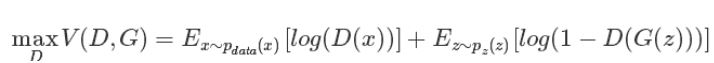
\includegraphics[scale=0.5]{img/p2.jpg}
	\caption{重建Loss}
\end{figure}

一个是判别器的判别Loss,判别器尽可能准确的区分真实图片与伪造图片。
\begin{figure}[H]
	\centering
	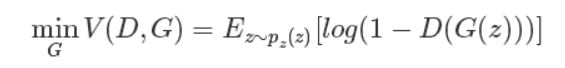
\includegraphics[scale=0.5]{img/p3.jpg}
	\caption{判别Loss}
\end{figure}

GAN的核心是一个最大最小化问题,包含对生成模型以假乱真的优化以及对判别模型的优化。
\begin{figure}[H]
	\centering
	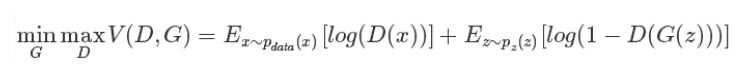
\includegraphics[scale=0.5]{img/p1.jpg}
	\caption{最大最小化问题}
\end{figure}

\subsection{CycleGAN原理}

CycleGAN是基于GAN实现的,它包含两个镜像对称的GAN,构成一个环形网络。
两个GAN共享两个生成器并各带一个判别器,总共4个Loss,并使用均方误差损失表示损失函数。

\begin{figure}[H]
	\centering
	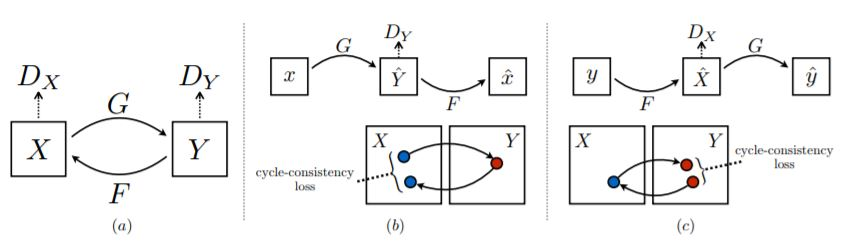
\includegraphics[scale=0.5]{img/p4.jpg}
	\caption{CycleGAN结构及损失定义}
\end{figure}


\begin{figure}[H]
	\centering
	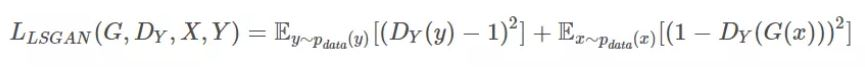
\includegraphics[scale=0.5]{img/p5.jpg}
	\caption{均方误差损失}
\end{figure}

\paragraph{生成器结构}
首先使用3层的CNN卷积神经网络层对图片的特征进行提取,
然后使用6层的Resnet深度残差网络将图像的特征转换到另一个分布上,并保留原始输入图片的特征,
最后使用反卷积神经网络层从特征向量中还原出图片

\paragraph{判别器结构}
主要为使用卷积神经网络从图片中提取特征,再通过一维输出的卷积层对提取出的特征进行判别

\section{实验}

\subsection{数据集}

实验中使用apple2orange及maps数据集进行模型训练和比较分析。

apple2orange数据集包含一系列 $256 \times 256$ 的苹果和橙子的图片用于风格迁移。

\begin{figure}[H]
	\centering
	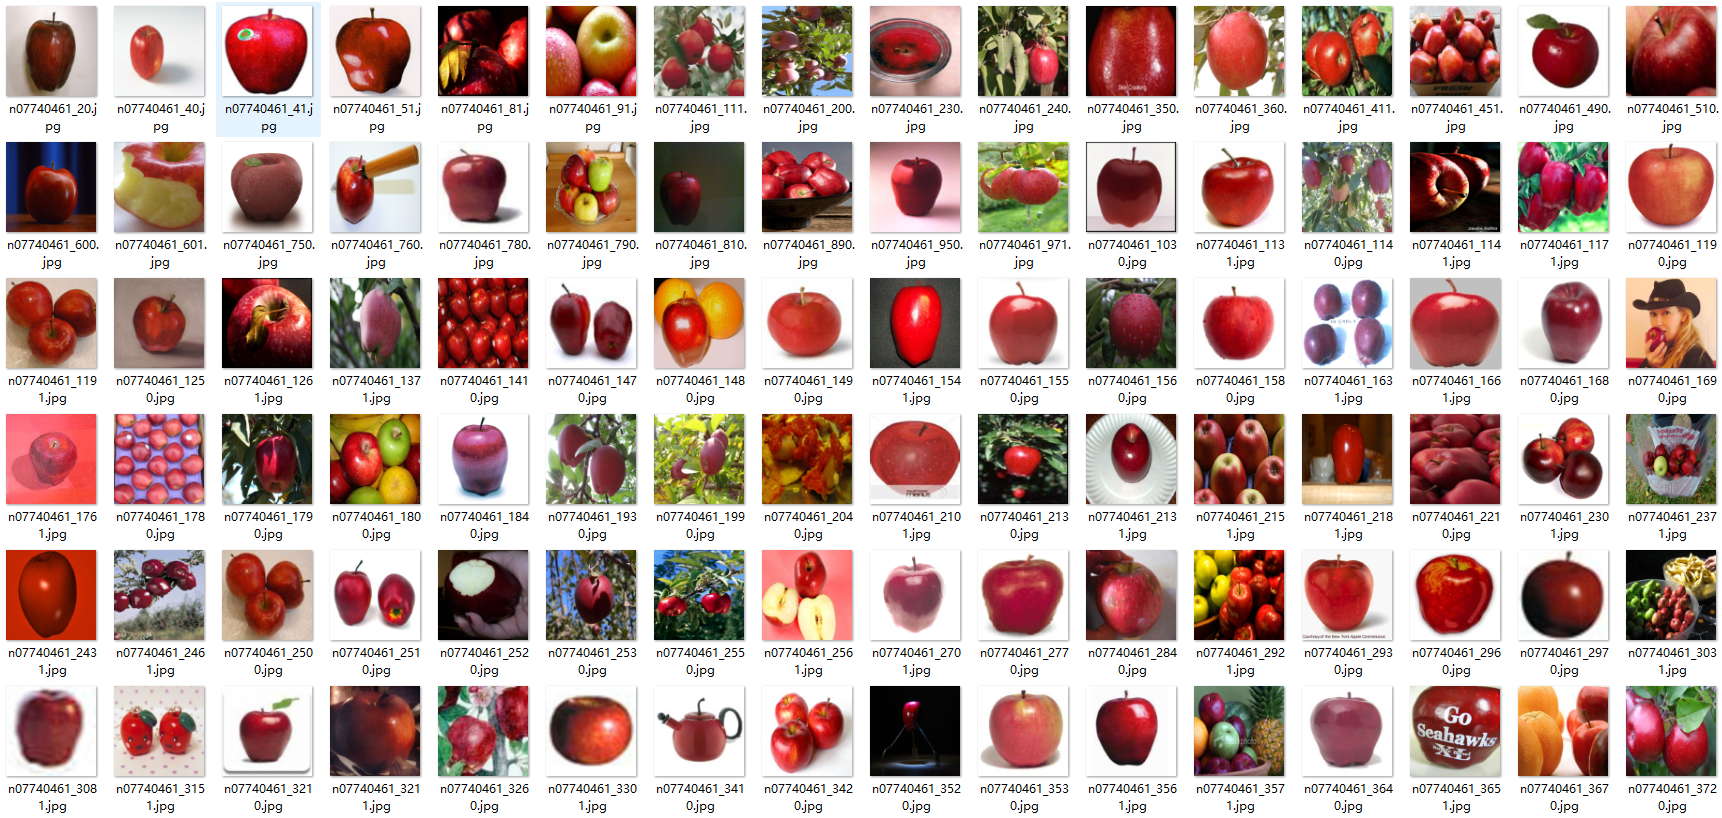
\includegraphics[width=8cm]{PIC/dataSet1.PNG}
	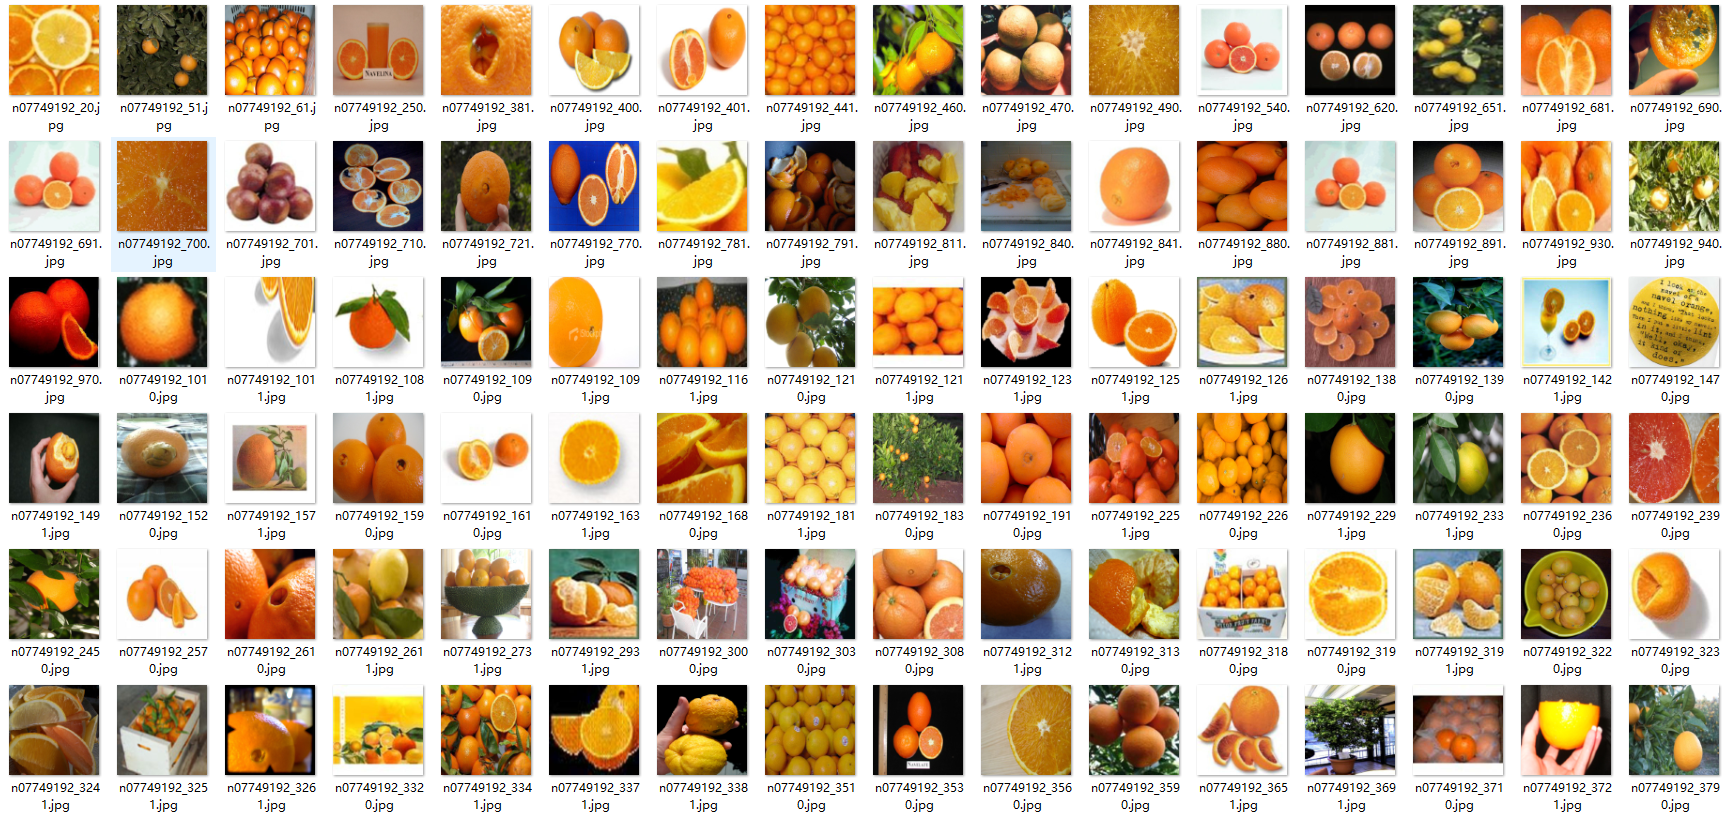
\includegraphics[width=8cm]{PIC/dataSet2.PNG}
	\caption{apple2orange训练集}
\end{figure}

maps数据集包含一系列 $256 \times 256$ 的卫星地图及手工绘制地图风格迁移。

\begin{figure}[H]
	\centering
	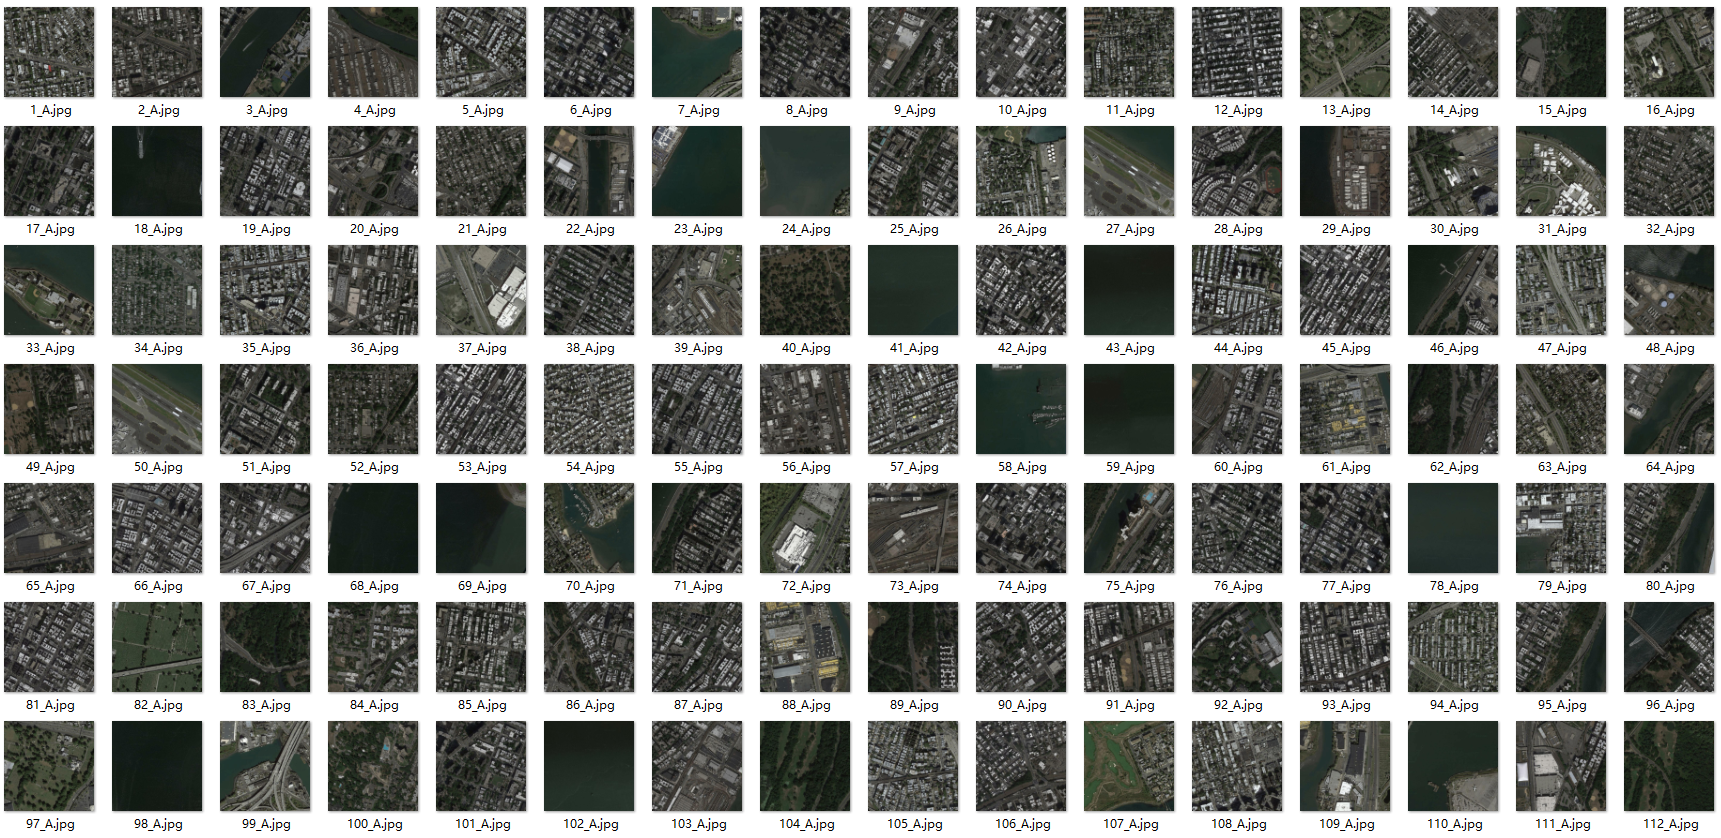
\includegraphics[width=8cm]{PIC/dataSet3.PNG}
	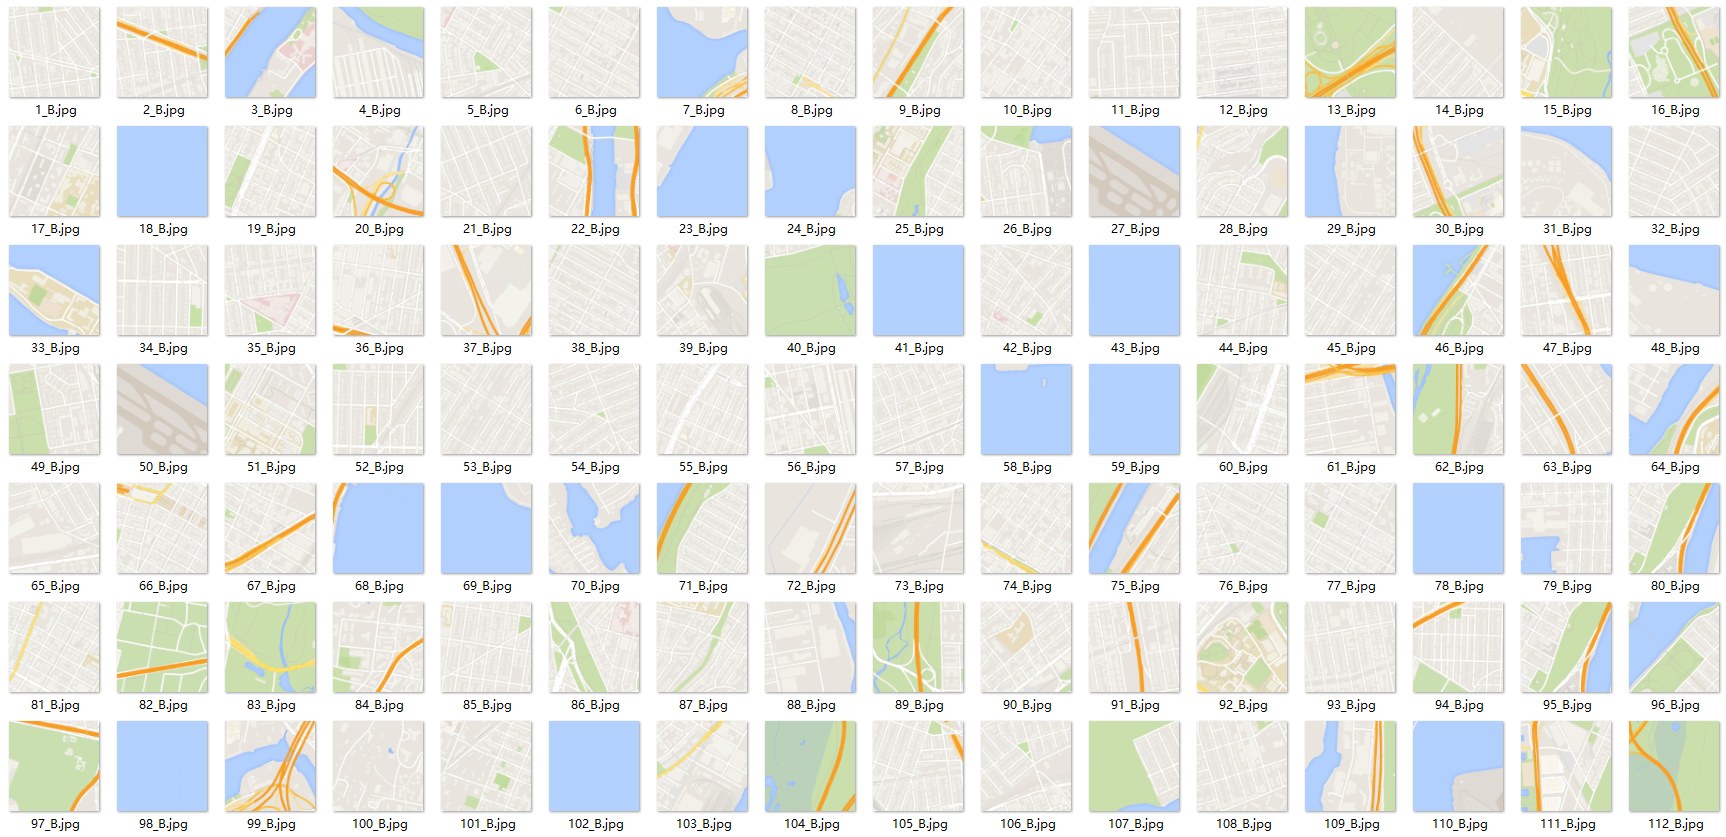
\includegraphics[width=8cm]{PIC/dataSet4.PNG}
	\caption{maps训练集}
\end{figure}

训练过程中使用了CPU R5 2600 + GPU RTX2060进行模型训练。

\subsection{fastNeuralStyle}

\paragraph{训练特点}需要拿一张图片作为风格进行特征提取,再选取被迁移的图片进行风格迁移,要进行两种风格的互相迁移则需要训练两个模型。

\paragraph{训练时间} 对于一张 $256 \times 256$ 的图片,每一个epoch需要约1个小时。训练2个epoch。

\subsection{CycleGAN}

\paragraph{训练特点} 需要拿两组图片进行训练,训练的图片不需要成对,训练出来的模型可以进行两种风格的迁移。

\paragraph{训练时间} 取决于训练集的大小及图片大小,对于一组2000张256X256的图片,每个epoch需要约60秒。训练20个epoch。

\subsection{训练结果}

\begin{figure}[H]
	\centering
	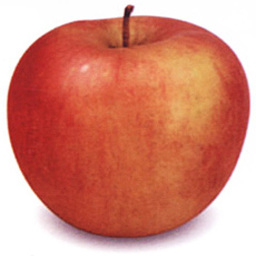
\includegraphics[width=2cm]{PIC/apple2orange/n07740461_1190_real_A.png}
	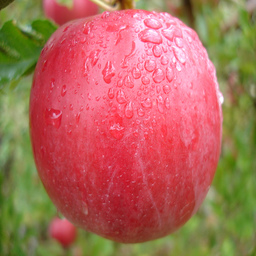
\includegraphics[width=2cm]{PIC/apple2orange/n07740461_10571_real_A.png}
	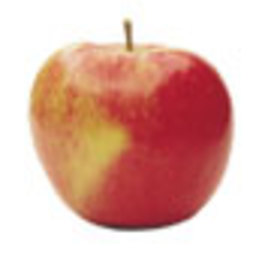
\includegraphics[width=2cm]{PIC/apple2orange/n07740461_12300_real_A.png}
	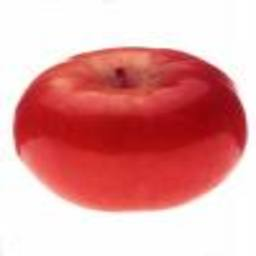
\includegraphics[width=2cm]{PIC/apple2orange/n07740461_12360_real_A.png}
	\caption{apple部分测试图片}
\end{figure}

\begin{figure}[H]
	\centering
	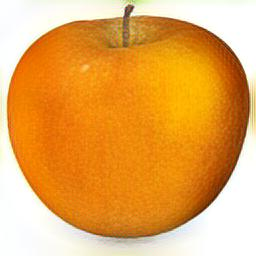
\includegraphics[width=2cm]{PIC/apple2orange/oa1.jpg}
	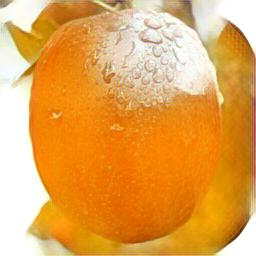
\includegraphics[width=2cm]{PIC/apple2orange/oa2.jpg}
	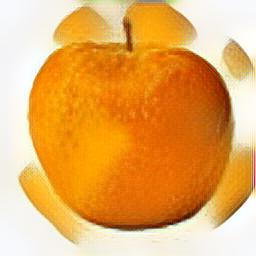
\includegraphics[width=2cm]{PIC/apple2orange/oa3.jpg}
	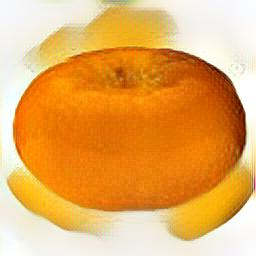
\includegraphics[width=2cm]{PIC/apple2orange/oa4.jpg}
	\caption{fastNeuralStyle风格迁移效果orange->apple}
\end{figure}

\begin{figure}[H]
	\centering
	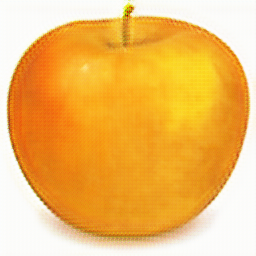
\includegraphics[width=2cm]{PIC/apple2orange/n07740461_1190_fake_B.png}
	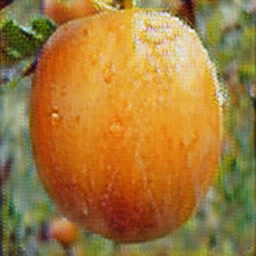
\includegraphics[width=2cm]{PIC/apple2orange/n07740461_10571_fake_B.png}
	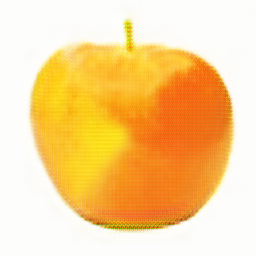
\includegraphics[width=2cm]{PIC/apple2orange/n07740461_12300_fake_B.png}
	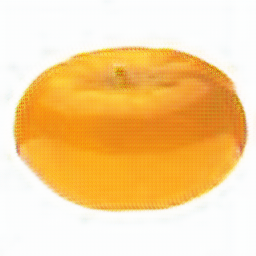
\includegraphics[width=2cm]{PIC/apple2orange/n07740461_12360_fake_B.png}
	\caption{CycleGAN风格迁移效果orange->apple}
\end{figure}

\begin{figure}[H]
	\centering
	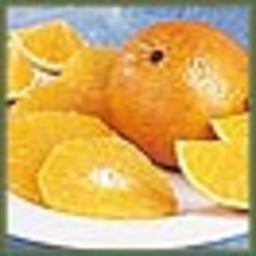
\includegraphics[width=2cm]{PIC/apple2orange/n07740461_1190_real_B.png}
	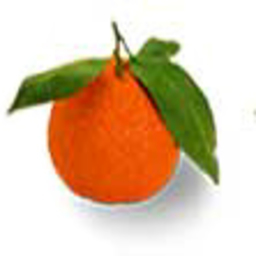
\includegraphics[width=2cm]{PIC/apple2orange/n07740461_10571_real_B.png}
	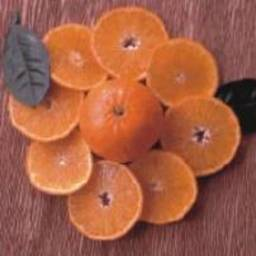
\includegraphics[width=2cm]{PIC/apple2orange/n07740461_12300_real_B.png}
	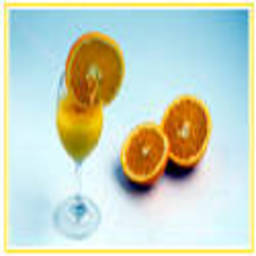
\includegraphics[width=2cm]{PIC/apple2orange/n07740461_12360_real_B.png}
	\caption{orange部分测试图片}
\end{figure}

\begin{figure}[H]
	\centering
	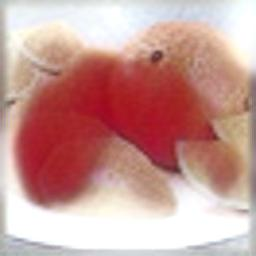
\includegraphics[width=2cm]{PIC/apple2orange/ao1.jpg}
	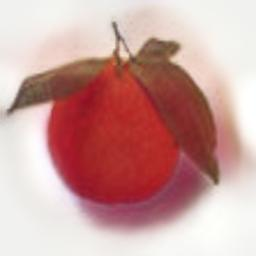
\includegraphics[width=2cm]{PIC/apple2orange/ao2.jpg}
	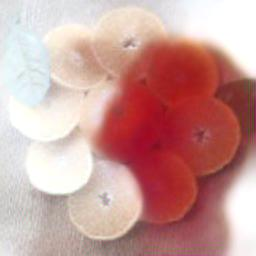
\includegraphics[width=2cm]{PIC/apple2orange/ao3.jpg}
	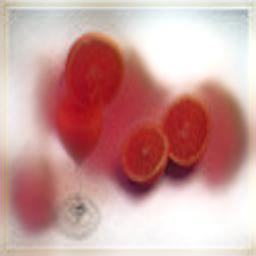
\includegraphics[width=2cm]{PIC/apple2orange/ao4.jpg}
	\caption{fastNeuralStyle风格迁移效果apple->orange}
\end{figure}


\begin{figure}[H]
	\centering
	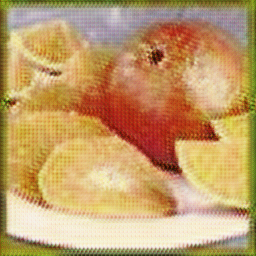
\includegraphics[width=2cm]{PIC/apple2orange/n07740461_1190_fake_A.png}
	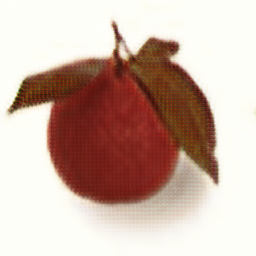
\includegraphics[width=2cm]{PIC/apple2orange/n07740461_10571_fake_A.png}
	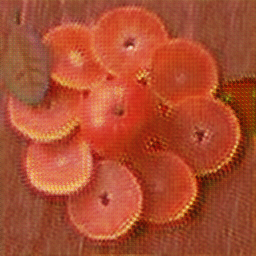
\includegraphics[width=2cm]{PIC/apple2orange/n07740461_12300_fake_A.png}
	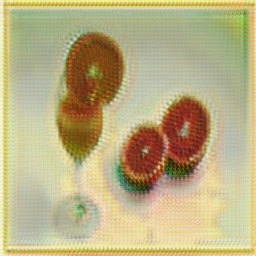
\includegraphics[width=2cm]{PIC/apple2orange/n07740461_12360_fake_A.png}
	\caption{CycleGAN风格迁移效果apple->orange}
\end{figure}


\begin{figure}[H]
	\centering
	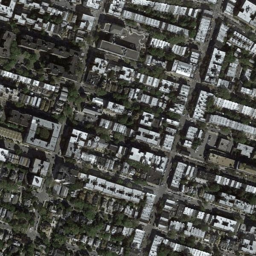
\includegraphics[width=2cm]{PIC/maps/1033_A_real_A.png}
	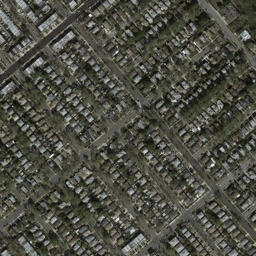
\includegraphics[width=2cm]{PIC/maps/1037_A_real_A.png}
	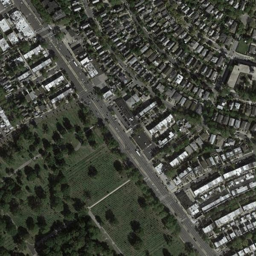
\includegraphics[width=2cm]{PIC/maps/1039_A_real_A.png}
	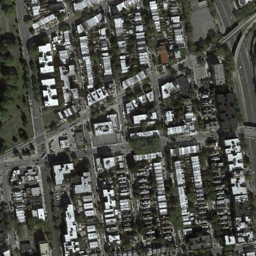
\includegraphics[width=2cm]{PIC/maps/1041_A_real_A.png}
	\caption{maps卫星图片部分测试图片}
\end{figure}

\begin{figure}[H]
	\centering
	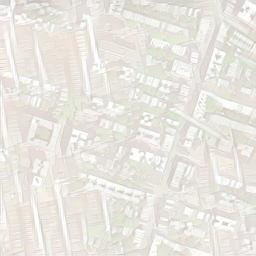
\includegraphics[width=2cm]{PIC/maps/pam1.jpg}
	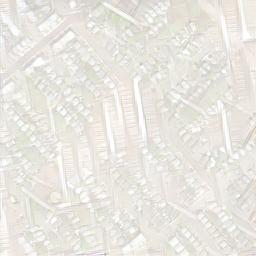
\includegraphics[width=2cm]{PIC/maps/pam2.jpg}
	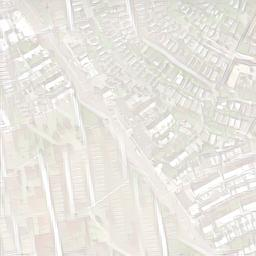
\includegraphics[width=2cm]{PIC/maps/pam3.jpg}
	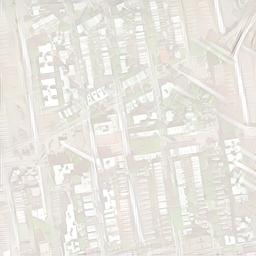
\includegraphics[width=2cm]{PIC/maps/pam4.jpg}
	\caption{fastNeuralStyle风格迁移效果绘制图片->卫星图片}
\end{figure}

\begin{figure}[H]
	\centering
	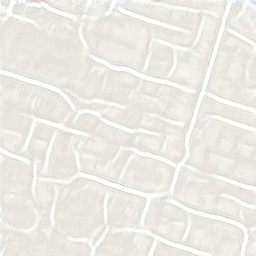
\includegraphics[width=2cm]{PIC/maps/1033_A_fake_B.png}
	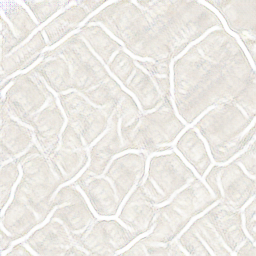
\includegraphics[width=2cm]{PIC/maps/1037_A_fake_B.png}
	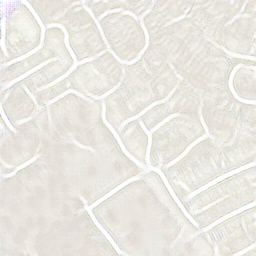
\includegraphics[width=2cm]{PIC/maps/1039_A_fake_B.png}
	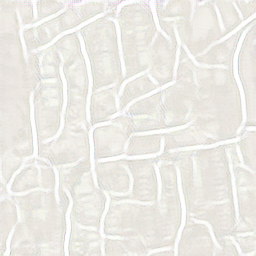
\includegraphics[width=2cm]{PIC/maps/1041_A_fake_B.png}
	\caption{CycleGAN风格迁移效果绘制图片->卫星图片}
\end{figure}

\begin{figure}[H]
	\centering
	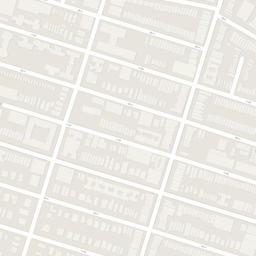
\includegraphics[width=2cm]{PIC/maps/1033_A_real_B.png}
	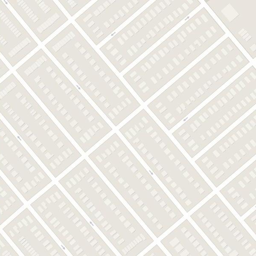
\includegraphics[width=2cm]{PIC/maps/1037_A_real_B.png}
	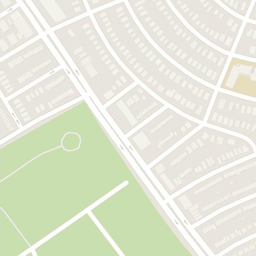
\includegraphics[width=2cm]{PIC/maps/1039_A_real_B.png}
	\includegraphics[width=2cm]{PIC/maps/1041_A_real_B.png}
	\caption{maps绘制图片部分测试图片}
\end{figure}

\begin{figure}[H]
	\centering
	\includegraphics[width=2cm]{PIC/maps/map1.jpg}
	\includegraphics[width=2cm]{PIC/maps/map2.jpg}
	\includegraphics[width=2cm]{PIC/maps/map3.jpg}
	\includegraphics[width=2cm]{PIC/maps/map4.jpg}
	\caption{fastNeuralStyle风格迁移效果卫星图片->绘制图片}
\end{figure}


\begin{figure}[H]
	\centering
	\includegraphics[width=2cm]{PIC/maps/1033_A_fake_A.png}
	\includegraphics[width=2cm]{PIC/maps/1037_A_fake_A.png}
	\includegraphics[width=2cm]{PIC/maps/1039_A_fake_A.png}
	\includegraphics[width=2cm]{PIC/maps/1041_A_fake_A.png}
	\caption{CycleGAN风格迁移效果卫星图片->绘制图片}
\end{figure}

\subsection{风格迁移效果对比}

fastNeuralStyle在对图片进行风格迁移时,容易产生过度迁移,如orange->apple的迁移上,第2,3,4张图中背景被添加上了橙色块,卫星图片->绘制图片上,第3,4张图中的草坪以及街区被额外添加上了一些物体。可能对图片特征识别不够准确,如apple->orange中对第1,3,4张图片迁移苹果的红色特征时迁移的不准确。

相比之下CycleGAN不易过度迁移以及风格迁移失准,但是CycleGAN在apple-orange上第1,4图片上的风格迁移略有不足,橙子并没有完全变红。

\section{结论}

在上述实验结果中,我们可以看到,在图像生成上,比起传统的 Neural Algorithm ,CycleGAN 无论是在效率上还是效果上,都要更加优秀。这种方法的发现,给 CycleGAN 带来新的应用场景,为无监督学习的发展贡献了一份力量。未来,CycleGAN 可能将成为艺术创作中的重要部分,只凭一部手机,就能完成拍照和风格变换,最终创作出一张极具风格的艺术作品。

另外,在大多数情况下,不成对的数据数量比成对的数据多非常多,它们应该被充分利用。本文的工作推动了无监督学习的发展,使得我们人类不必再为数据做配对,“自动地”根据不成对的数据完成风格的学习。


\begin{thebibliography}{00}
\bibitem{b6} E. L. Denton, S. Chintala, R. Fergus, et al. Deep gen- erative image models using a laplacian pyramid of ad- versarial networks. In NIPS, 2015.
\bibitem{b13} L. A. Gatys, A. S. Ecker, and M. Bethge. Image style transfer using convolutional neural networks. CVPR, 2016.
\bibitem{b16} I. Goodfellow, J. Pouget-Abadie, M. Mirza, B. Xu, D. Warde-Farley, S. Ozair, A. Courville, and Y. Ben- gio. Generative adversarial nets. In NIPS, 2014.
\bibitem{b23} J. Johnson, A. Alahi, and L. Fei-Fei. Perceptual losses for real-time style transfer and super-resolution. In ECCV, 2016.
\bibitem{b24} Z. Kalal, K. Mikolajczyk, and J. Matas. Forward- backward error: Automatic detection of tracking fail- ures. In ICPR, 2010.
\bibitem{b48} N. Sundaram, T. Brox, and K. Keutzer. Dense point trajectories by gpu-accelerated large displacement op- tical flow. In ECCV, 2010.
\bibitem{b66} J.-Y. Zhu, P. Kra ̈henbu ̈hl, E. Shechtman, and A. A. Efros. Generative visual manipulation on the natural image manifold. In ECCV, 2016.
\end{thebibliography}

\end{document}
